\documentclass[a4paper,11pt]{article}
\usepackage[frenchb]{babel}
\usepackage[T1]{fontenc}
\usepackage[utf8]{inputenc}
\usepackage{lmodern}
\usepackage{microtype}

\usepackage{array,multirow,makecell}
\setcellgapes{1pt}
\makegapedcells
\usepackage{caption}
\usepackage{adjustbox}

\usepackage{amsmath,amssymb,bm,upgreek,stmaryrd,mathrsfs,systeme}

\usepackage{graphicx}

\usepackage{geometry}
\geometry{hmargin=3cm,vmargin=2cm}

\usepackage{hyperref}

\title{Deuxième modèle de la Terre comme système énergétique}

\begin{document}
\maketitle

\section{Description du modèle}

\subsection{Modèle 1}

On part des données suivantes :

\begin{enumerate}

\item[•] Puissance surfacique du Soleil reçu par la Terre : $P_S = 1300 ~ W \cdot m^{-2}$
\item[•] Rayon de la Terre : $R_T$ = 6371 km
\item[•] Constante de Stefan-Boltzmann : $\sigma = 5,67 \cdot 10^{-8} ~ W \cdot m^{-2} \cdot K^4$ 
\item[•] Période de rotation de la Terre : T = 1 jour (donc $\omega = \dfrac{2\pi}{T}$ pulsation propre de la Terre)

\end{enumerate}

Pour commencer, la puissance que reçoit la Terre correspond au produit de la puissance surfacique et de la surface de la Terre en considérant que la surface de la Terre est un disque pour connaître la puissance réelle reçue sur l'ensemble de sa surface. En notant $P_S$ la puissance surfacique du Soleil à la distance Terre-Soleil du Soleil, $P_{S/T}$ la puissance reçue par la Terre, S la surface du maître-couple (voir Table 1 dans Annexes) de la Terre et $R_T$ le rayon de la Terre, on a :

\[ P_{S/T} = P_S \cdot S = P_S \cdot \pi R_T^2  \]

Ensuite, en considérant que l'albédo moyen de la Terre est $A = 0.3$, on obtient que la puissance réfléchie $P_r$ par la surface terrestre est :

\[ P_r = A \cdot P_{S/T} \]

En utilisant la loi de Stefan-Boltzmann, on connaît la puissance émise par la Terre $P_e$ :

\[ P_e = \sigma T^4 \cdot 4 \pi R^2 \]

Dans ce modèle, nous négligeons les effets internes de la Terre, ce qui implique que celle-ci n'émet de puissance que par ce qu'elle reçoit du Soleil, soit la puissance absorbée modélisée par la loi de Stefan-Boltzmann. On considère alors que la puissance reçue par la Terre $P_{S/T}$ est égale à la somme de la puissance réfléchie $P_r$ et de la puissance émise $P_e$ :

\[ P_{S/T} = P_r + P_e \]

Finalement, en remplaçant par les expressions explicitées précédemment et en isolant la température de la Terre $T$, on obtient :

\[ T = \left(\dfrac{(1 - A) \cdot P_S}{4\sigma}\right)^{1/4} \]

\subsection{Modèle 2}

Dans ce modèle, on propose une amélioration du premier modèle proposé en considérant la position sur Terre (latitude et longitude), ainsi que le temps, c'est-à-dire la partie de la Terre qui est éclairée par le Soleil.

On considère que la Terre suit une trajectoire circulaire. Le rayonnement du soleil arrivant sur la terre est supposé orthogonal (Terre à une distance infinie du Soleil). On ne prend pas encore en compte l’atmosphère. L’albédo est considéré comme une constante A. On prend en compte la latitude et la longitude ainsi que la rotation de la Terre en se basant sur le méridien de Greenwich (heure 0). On néglige l'inclinaison de la Terre.

\textbf{Image à inclure ici ! ! !
}

Dans ce modèle, la puissance reçue par un élément de surface de la Terre est $P_S \cdot \overrightarrow{dS'}$. De plus, on a $\overrightarrow{dS} = dS \cdot \vec{n}$ et $\overrightarrow{dS'} = dS' \cdot \vec{n'}$. Ainsi, la puissance surfacique reçue par un élément de surface de la Terre est :

\[ P_{S, reçue} = \dfrac{P_S \cdot \overrightarrow{dS} \cdot \overrightarrow{dS'}}{dSdS'} \]

Ce qui donne en simplifiant :

\[ P_{S,reçue} = P_S \cdot \vec{n} \cdot \vec{n'} \]

On projette ensuite $\vec{n}$ et $\vec{n'}$ dans le repère cartésien (x(t), y(t)). Chaque axe dépend de t en raison de la rotation de la Terre sur elle-même, mais ces deux-là sont immobiles dans référentiel de la Terre.

\textbf{Modéliser la situation !!!}

Puisque $ \vec{n} = -\overrightarrow{e_r}$, on a :

\[ \vec{n} = - \sin \theta \cos \phi ~ \vec{x} - \sin \theta \sin \phi ~ \vec{y} \]

En considérant la période de la Terre, on a une projection de $\vec{n'}$ qui va dépendre du temps ($\vec{n'}$ immobile dans le référentiel héliocentrique). Cette projection est la suivante :

\[ \vec{n'} = - \cos \omega t ~ \vec{y} - \sin \omega t ~ \vec{x} \]

Finalement :

\[ P_{S,reçue} = P_S \cdot (- \sin \theta \cos \phi ~ \vec{x} - \sin \theta \sin \phi ~ \vec{y}) \cdot (- \cos \omega t ~ \vec{y} - \sin \omega t ~ \vec{x}) \]

D'où :

\[ P_{S,reçue} = P_S \cdot (\sin \omega t \cdot \sin \theta \cos \phi + \cos \omega t \cdot \sin \theta \sin \phi) \]

Le but étant de rentrer la latitude et la longitude pour déterminer la température en un point de la Terre, on a :

\[ lat = \phi \]
\[ long = \dfrac{\pi}{2} - \theta \leftrightarrow \theta = \dfrac{\pi}{2} - long \]

On peut ensuite calculer la température en un point de la Terre, en fonction de la longitude, la latitude et l'heure de la journée :

\[ T (\theta , \phi , t) = \left(\dfrac{(1 - A) \cdot P_{S,reçue}}{4\sigma}\right)^{1/4} \]

\section{Annexes}

\begin{adjustbox}{center}
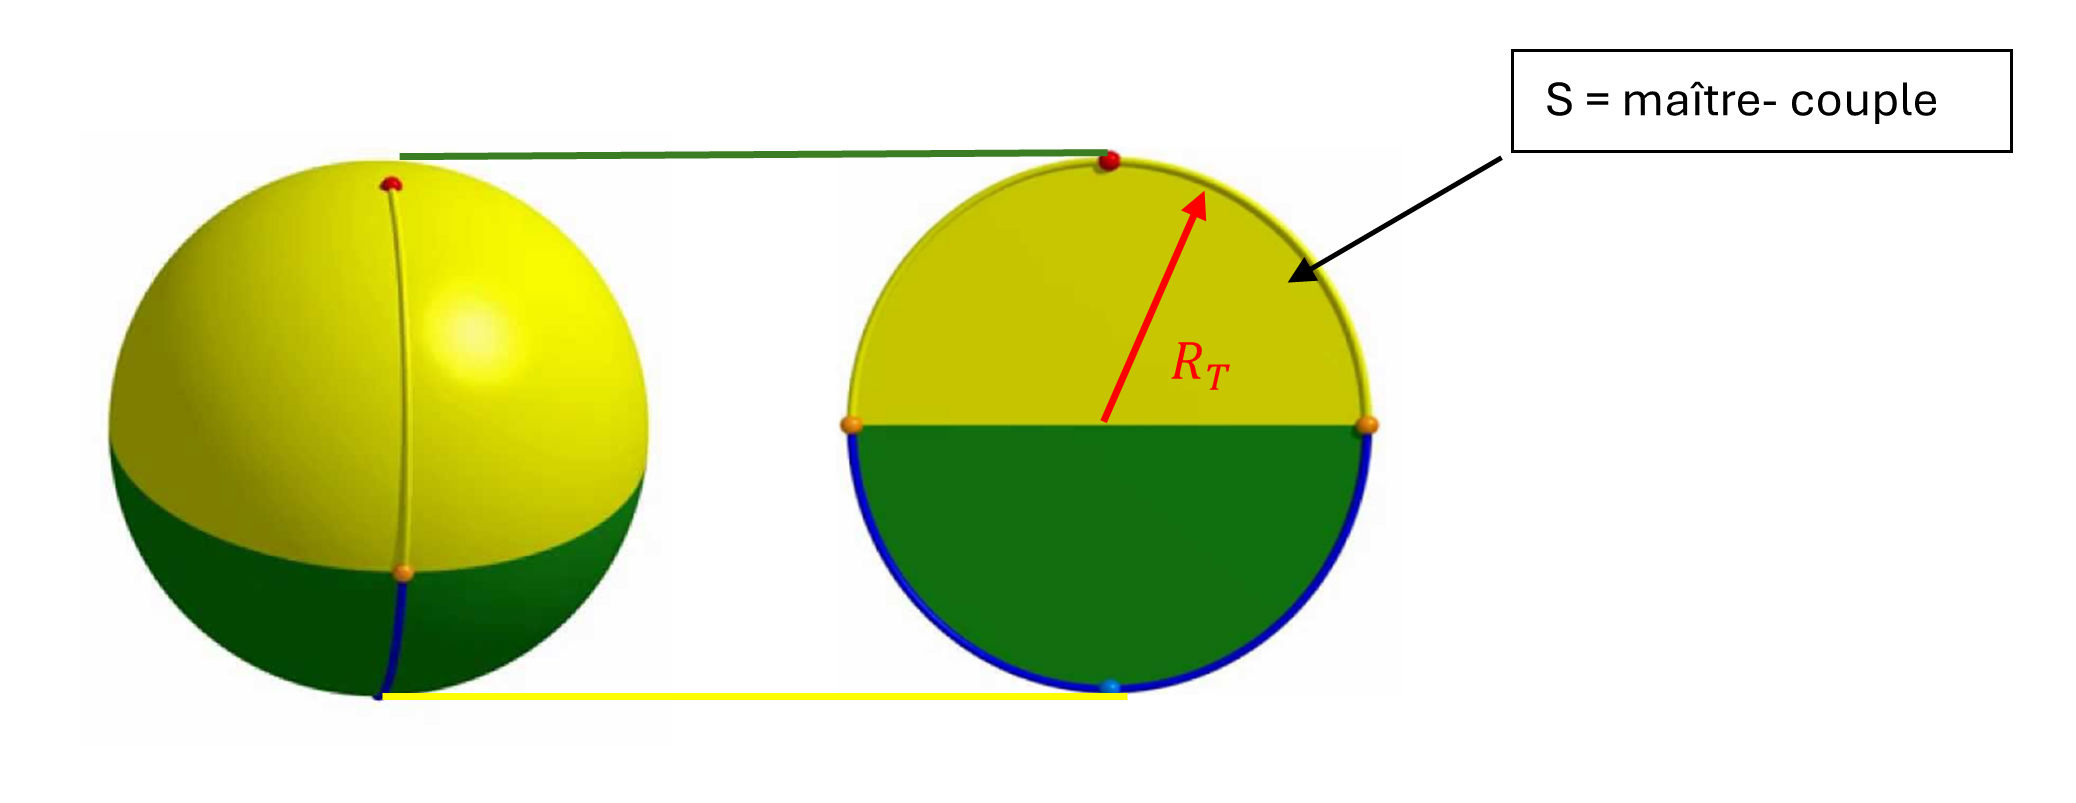
\includegraphics[scale=0.9]{Schema_maitre_couple}
\end{adjustbox}
\captionof{table}{Surface considérée (maître-couple) \\} 

Dans ce modèle, on propose une amélioration du premier modèle proposé en considérant la position sur Terre (latitude et longitude), ainsi que le temps, c'est-à-dire la partie de la Terre qui est éclairée par le Soleil.

On considère que la Terre suit une trajectoire circulaire. Le rayonnement du soleil arrivant sur la terre est supposé orthogonal (Terre à une distance infinie du Soleil). On ne prend pas encore en compte l'atmosphère. L'albédo est considéré comme une constante A. On prend en compte la latitude et la longitude ainsi que la rotation de la Terre en se basant sur le méridien de Greenwich (heure 0). On néglige l'inclinaison de la Terre.





























\end{document}